% !TeX spellcheck = en_GB

\section{Introduction}\label{Introduction}

\subsection{Motivation}
Every year, lecturer in the field of theoretical computer science or an related one face the task to create the 4-tuple exam $exercise = (grammar,\ word,\ parse\ table,\ derivation\ $ $tree)$ that tests if their students have understood the way of working of the Cocke-Younger-Kasami (CYK) algorithm. For it exercises need to be created which is a bit of a time consuming task. \\
Various implementations and small online tools of the CYK algorithm can be found \footnote{\href{http://lxmls.it.pt/2015/cky.html}{CYK online tool: http://lxmls.it.pt/2015/cky.html}} \footnote{\href{http://jflap.org/tutorial/grammar/cyk/index.html}{CYK parser implementation: http://jflap.org/tutorial/grammar/cyk/index.html}} \footnote{\href{https://github.com/ajh17/CYK-Java}{CYK algorithm implementation in Java: https://github.com/ajh17/CYK-Java}} but none actually assists during the process of creating an exercise.\\
Therefore algorithms are needed to generate specifically suitable exercises with a high chance of success. Also a GUI tool, that allows automatic generation of the suitable exam exercises and further modification, is required and so a own solution is implemented.

\subsection{Context Free Grammar} \label{cfgChapter}
Firstly, we define a Context Free Grammar (CFG) as follows:
\begin{DefGrey} \textbf{Context Free Grammar (CFG)}\\
	A CFG is a 4-tuple $G=(V,\ \Sigma,\ S,\ P)$:
	\begin{itemize}
		\item $V$ is a finite set of variables.
		\item $\Sigma$ is an alphabet
		\item $S$ is the start symbol and $S \in V$.
		\item $P$ is a finite set of rules: $P \subseteq V \times (V \cup \Sigma)^{*}$.
	\end{itemize}
	It holds: $\Sigma \cap V =  \emptyset$.
\end{DefGrey}
\noindent Secondly, we define a CFG with restrictions (CFGR) as:
\begin{DefGrey}\label{CFGinCNF} \textbf{CFG with restrictions (CFGR)}\\
	A CFG $G=(V,\ \Sigma,\ S,\ P)$ is a CFGR if:
	\begin{itemize}
		\item $P \subseteq V \times (V^2 \cup \Sigma)$.~
	\end{itemize}
\end{DefGrey}
\noindent Throughout this thesis a grammar is always synonymous with Definition \ref{CFGinCNF}. Note that a CFGR is not necessarily in chomsyk normal form (CNF) because it is still possible that there are unreachable variables \textendash~from the starting variable \textendash~ or useless rules. For further convenience the following default values are always assumed in this thesis:
\begin{itemize}
	\item $V = \{A, B, ...\}=:Lhse.$
	\item $(V^2 \cup\ \Sigma)=\{AA, AB, BB, BA, BS, AC, ... \} \cup \{a, b, ...\}=:Rhse.$
\end{itemize}
A rule consists of a left hand side element ($lhse \in Lhse$) and a right hand side element ($rhse \in Rhse$). \\
\begin{testexample}[lhse and rhse]
	$lhse \longrightarrow rhse$ applied to $A \longrightarrow c$ and $B \longrightarrow AC$ means that $A$ and $B$ are a $lhse$ and $c$ and $AC$ are a $rhse$. Elements of $V^2$ are often referred to as variable compounds.
\end{testexample}~\\
For a word and a sub word Definition \ref{word} holds:
\begin{DefGrey} \label{word} \textbf{Word $\mathbf{w}$ and sub word}
	\begin{itemize}[leftmargin=1cm]
		\item Word $w$:~~~$w = w_0\cdot w_1\cdot ...\cdot w_j$ and $w \in \Sigma^*$.
		\item Sub word $sw$ of a word $w$:~~~$sw = w_k\cdot ...\cdot w_{l+k}$ where $0\leq i$ and $l+k \leq j$.
	\end{itemize}
\end{DefGrey}
\noindent For a language and a language over a grammar Definition \ref{wordLanguage} holds:
\begin{DefGrey}\label{wordLanguage} \textbf{Language $L$ and language $\mathbf{L(G)}$}~
	\begin{itemize}[leftmargin=1cm]
		\item Language $L$:~~~$L$ is a language over an alphabet $\Sigma$ that is subset of $\Sigma^*$, that is a set of words over that alphabet. 
		\item Language $L(G)$:~~~$L(G)$ is the language over a grammar $G$, that describes the set of words over that alphabet.
	\end{itemize}
\end{DefGrey}
\noindent Moreover in the context of talking about sets, a set is always described beginning with an upper case letter, while one specific element of a set is described beginning with a lower case letter. \\
\begin{testexample}[Upper Case Letter for sets]
	Example: A "$Pyramid$" is a set consisting of multiple "$Cell$"s, whereas a $Cell$ is again a subset of the set of variables "$V$". A "$cellElement$" is one specific element of a "$Cell$". (For further explanation behind this specific example see chapter \ref{dataStructurePyramid})
\end{testexample}~\\


\pagebreak
\subsection{General approaches of parsing} \label{approaches}
Next, the basic approach that may help finding a good algorithm is explained informally analogous to \cite{Duda.2012}. At first, parsing is described in general and afterwards its two characteristics are explained.  
\begin{DefGrey}
	\textbf{Backward Problem = Parsing ($\mathbf{w\overset{?}{\in}L(G)}$)}\\
	Input: $w$ and a grammar $G$. \\
	Output: $w \in L(G) \Longrightarrow$ derivation $d$.
\end{DefGrey}
\noindent It is called parsing if there is a word $w$ given and it is of interest to know if it is element of $L(G)$. Parsing is also the basis of the Cocke-Younger-Kasami algorithm.\\
After having defined what parsing in general is, it is important to know the two different ways of parsing, that will act as an idea provider for the algorithms.
\begin{mdframed}[backgroundcolor=defColour]
	\textbf{Bottom-Up parsing} \\
Bottom-Up parsing means to start parsing from the leaves up to the root node.
\end{mdframed}
\noindent Actually, Bottom-Up parsing is the method used in the Cocke-Younger-Kasami algorithm, which fills the parse table from the "bottom up"\cite{Duda.2012}.\\
Bottom-up parsing starts by recognizing the words smallest sub words before its mid-size sub words, and leaving the largest overall word as the last.
\begin{mdframed}[backgroundcolor=defColour]
	\textbf{Top-Down parsing} \\
	 Top-Down parsing means to start parsing from the root node down to the leaves.
\end{mdframed}
\noindent "Top-Down parsing starts with the root node and successively applies rules from $P$, with the goal of finding a derivation of the test sentence $w$." \cite{Duda.2012} (The so called test sentence is synonymous to an word $w$.)
\pagebreak
\subsection{Data Structure Pyramid} \label{dataStructurePyramid}
To be able to describe how the different algorithms work in a simpler way, the help data structure $Pyramid$ is defined \textendash~note that $Pyramid$ is a set and starts with upper case.
\begin{DefGrey} \textbf{$Pyramid$} \\
	$Pyramid :=\{ Cell_{i,j}\ |\ i \in [0,\ i_{max}],\  j \in [0,\ j_{max,i}],\ i_{max} = |w|-1,~j_{max,i} = i_{max} -i\}$\\
	~~~where $Cell_{i,j} \subseteq \{(V,k)~|~k \in \mathbb{N} \}$ denotes the contents of the j'th cell in row i\\
	~~~and $[i,\ j] := \{i,\ i+1,..., j-1,\ j\} \subseteq \mathbb{N}$.
\end{DefGrey}
\noindent The cell $Cell_{i_{max},0}$ is called the root of such a $Pyramid$ and Figure \ref{visualPyramid} shows the visual representation of one.
\newcommand{\boxpyramid}[1]{
	\fontsize{5}{12}\selectfont{#1}
}
\begin{figure}[H]
\centering
\label{visualPyramid}
	\resizebox{\linewidth}{!}{
		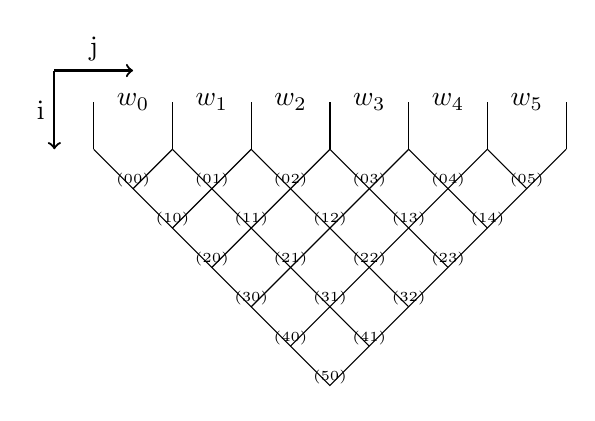
\begin{tikzpicture}[baseline]
		\newcommand{\myfontvars}[1]{
			\fontsize{4.9}{12}\selectfont{#1}
		}\newcommand{\myfontnumbering}[1]{
			\fontsize{2.5}{12}\selectfont{#1}
		}%Outer hull
		%Tip of the pyramid
		\coordinate (tip) at (3,-3);
		\foreach \i in {0,...,6} {
			\coordinate (\i) at (\i,0);
		}
		%\draw[help lines] (-1,1) grid (6,-3);
		\draw [->, thick] (-0.5,1) -- (0.5,1);
		\node [above] at (0, 1) {j};
		\draw [->, thick] (-0.5,1) -- (-0.5,-0.0);
		\node [left] at (-0.5,0.5) {i};
		%Draw the left and right line of the pyramid pointing downwards
		\draw (0) -- (tip) -- (6);
		%Grid lines direction down-left to top-right
		\coordinate (dl1) at (0.5,-0.5);
		\coordinate (dl2) at (1.0,-1.0);
		\coordinate (dl3) at (1.5,-1.5);
		\coordinate (dl4) at (2.0,-2.0);
		\coordinate (dl5) at (2.5,-2.5);
		\draw (dl1) -- (1,0);
		\draw (dl2) -- (2,0);
		\draw (dl3) -- (3,0);
		\draw (dl4) -- (4,0);
		\draw (dl5) -- (5,0);
		%Grid lines direction down-right to top-left
		\coordinate (dr1) at (3.5,-2.5);
		\coordinate (dr2) at (4.0,-2.0);
		\coordinate (dr3) at (4.5,-1.5);
		\coordinate (dr4) at (5.0,-1.0);
		\coordinate (dr5) at (5.5,-0.5);
		\draw (dr1) -- (1,0);
		\draw (dr2) -- (2,0);
		\draw (dr3) -- (3,0);
		\draw (dr4) -- (4,0);
		\draw (dr5) -- (5,0);
		%Small lines at the top
		\coordinate (top0) at (0.0,0.0);
		\coordinate (top1) at (1.0,0.0);
		\coordinate (top2) at (2.0,0.0);
		\coordinate (top3) at (3.0,0.0);
		\coordinate (top4) at (4.0,0.0);
		\coordinate (top5) at (5.0,0.0);
		\coordinate (top6) at (6.0,0.0);
		\coordinate (topUpper0) at (0.0,0.6);
		\coordinate (topUpper1) at (1.0,0.6);
		\coordinate (topUpper2) at (2.0,0.6);
		\coordinate (topUpper3) at (3.0,0.6);
		\coordinate (topUpper4) at (4.0,0.6);
		\coordinate (topUpper5) at (5.0,0.6);
		\coordinate (topUpper6) at (6.0,0.6);
		\draw (top0) -- (topUpper0);
		\draw (top1) -- (topUpper1);
		\draw (top2) -- (topUpper2);
		\draw (top3) -- (topUpper3);
		\draw (top4) -- (topUpper4);
		\draw (top5) -- (topUpper5);
		\draw (top6) -- (topUpper6);
		%The string
		\coordinate (w0) at (0.5,0.6);
		\coordinate (w1) at (1.5,0.6);
		\coordinate (w2) at (2.5,0.6);
		\coordinate (w3) at (3.5,0.6);
		\coordinate (w4) at (4.5,0.6);
		\coordinate (w5) at (5.5,0.6);
		\node [] at (w0) {$w_0$};
		\node [] at (w1) {$w_1$};
		\node [] at (w2) {$w_2$};
		\node [] at (w3) {$w_3$};
		\node [] at (w4) {$w_4$};
		\node [] at (w5) {$w_5$};
		% Variables in the cells
		%cell00
		\coordinate (center00) at (0.5,0.0);
		\node [below=0.18cm] at (center00) {\myfontnumbering{$(00)$}};
		%cell01
		\coordinate (center01) at (1.5,0.0);
		\node [below=0.18cm] at (center01) {\myfontnumbering{$(01)$}};
		%cell02
		\coordinate (center02) at (2.5,0.0);
		\node [below=0.18cm] at (center02) {\myfontnumbering{$(02)$}};
		%cell03
		\coordinate (center03) at (3.5,0.0);
		\node [below=0.18cm] at (center03) {\myfontnumbering{$(03)$}};
		%cell04
		\coordinate (center04) at (4.5,0.0);
		\node [below=0.18cm] at (center04) {\myfontnumbering{$(04)$}};
		%cell05
		\coordinate (center05) at (5.5,0.0);
		\node [below=0.18cm] at (center05) {\myfontnumbering{$(05)$}};
		%cell10
		\coordinate (center10) at (1.0,-0.5);
		\node [below=0.18cm] at (center10) {\myfontnumbering{$(10)$}};
		%cell11
		\coordinate (center11) at (2.0,-0.5);
		\node [below=0.18cm] at (center11) {\myfontnumbering{$(11)$}};
		%cell12
		\coordinate (center12) at (3.0,-0.5);
		\node [below=0.18cm] at (center12) {\myfontnumbering{$(12)$}};
		%cell13
		\coordinate (center13) at (4.0,-0.5);
		\node [below=0.18cm] at (center13) {\myfontnumbering{$(13)$}};
		%cell14
		\coordinate (center14) at (5.0,-0.5);
		\node [below=0.18cm] at (center14) {\myfontnumbering{$(14)$}};
		%cell20
		\coordinate (center20) at (1.5,-1.0);
		\node [below=0.18cm] at (center20) {\myfontnumbering{$(20)$}};
		%cell21
		\coordinate (center21) at (2.5,-1.0);
		\node [below=0.18cm] at (center21) {\myfontnumbering{$(21)$}};
		%cell22
		\coordinate (center22) at (3.5,-1.0);
		\node [below=0.18cm] at (center22) {\myfontnumbering{$(22)$}};
		%cell23
		\coordinate (center23) at (4.5,-1.0);
		\node [below=0.18cm] at (center23) {\myfontnumbering{$(23)$}};
		%cell30
		\coordinate (center30) at (2.0,-1.5);
		\node [below=0.18cm] at (center30) {\myfontnumbering{$(30)$}};
		%cell31
		\coordinate (center31) at (3.0,-1.5);
		\node [below=0.18cm] at (center31) {\myfontnumbering{$(31)$}};
		%cell32
		\coordinate (center32) at (4.0,-1.5);
		\node [below=0.18cm] at (center32) {\myfontnumbering{$(32)$}};
		%cell40
		\coordinate (center40) at (2.5,-2.0);
		\node [below=0.18cm] at (center40) {\myfontnumbering{$(40)$}};
		%cell41
		\coordinate (center41) at (3.5,-2.0);
		\node [below=0.18cm] at (center41) {\myfontnumbering{$(41)$}};
		%cell50
		\coordinate (center50) at (3.0,-2.5);
		\node [below=0.18cm] at (center50) {\myfontnumbering{$(50)$}};
		\end{tikzpicture}
	}
\caption{Visual representation of a $Pyramid$ with the word $w$ written above it.}
\end{figure}
\pagebreak
\subsection{ Cocke-Younger-Kasami Algorithm}
The Cocke-Younger-Kasami Algorithm (CYK) was independently developed in the 1960s by Itiroo Sakai \cite{Sakai.1962}, John Cocke and Jacob Schwartz \cite{JohnCockeJacobT.Schwartz.1970}, Tadao Kasami \cite{Kasami.1966} and Daniel Younger \cite{YOUNGER.1967}.\\
The idea is to find all possible derivations of each sub word starting with size one and to consecutively use this information to find all possible derivations with a larger size of the subword up to the size of $w$. Finally it is checked whether $w \in L(G)$ through the presence of the start variable in the root of the pyramid. \\
The description of the algorithm follows the source \cite{Hoffmann.2015} adjusted to the data structure $Pyramid$. 
Later on it can be seen that the CYK algorithm can be used as a basis to find good algorithms.\\

\noindent \frame{
	\begin{algorithm}[H] %or another one check
		\caption{CYK}
		\label{CYK}
		\SetAlgoLined
		\KwIn{Grammar $G=(V,\ \Sigma,\ S,\ P)$ and word $w \in \Sigma^* = \{w_0,~w_1,~...,~w_j\}$ }
		\KwOut{true $\Leftrightarrow w\in L(G)$}
		$Pyramid = \emptyset $\;
		\For{$j:=0 \to i_{max}$}{ \label{row1}
			$Pyramid = Pyramid~\cup \{(X,j+1)~|~X \longrightarrow w_j\}$; \tcp{Fills cells $Cell_{0,j}$} \label{fill1}
		}
		\For{$i:=1 \to i_{max}$}{ \label{rows}
			\For{$j:=0 \to j_{max,i}$}{ \label{eachCell}
				\For{$k:=i-1 \to 0$}{ \label{cykCellCombs}
					$Pyramid = Pyramid~\cup \{(X,k+j+1)\ |\ X\longrightarrow YZ,\ Y \in Cell_{k,j},\ Z \in Cell_{i-k-1,k+j+1} \}$; \tcp{Fills cells $Cell_{i,j}$ \label{fill2}}
				}
			}
		}
		\If{$(S,i) \in Cell_{i_{max},0}$}{ 
			\Return $true$; \label{true}
		}
		\Return $false$;
		\footnotetext{ 
		Line \ref{row1}: First row.\\
		Line \ref{rows}: All rows except the first. \\
		Line \ref{eachCell}: All cells in each row. \\
		Line \ref{cykCellCombs}: All possible cell combinations for each cell. \\
		Line \ref{true}: True if $Cell_{i_{max},0}$ contains the start variable.
		}
	\end{algorithm}
}
~
\begin{testexample}[Algorithm CYK]
During the execution of the CYK algorithm the parsing table is filled as shown in Figure \ref{exampleCYK}. At first the row with index $i=0$ is filled after Line 2 to Line 4 of the CYK algorithm, i.e. a $Cell_{0,j}$ will contain the variable if it has the terminal $w_j$ as its $rhse$. Then for each row $i$ every cell with index $j$ is looked at. Every possible combination of sub words for a cell are taken into account, i.e. for $Cell_{4,1}$ there are the combinations of ($Cell_{0,1},Cell_{3,2}$), ($Cell_{1,1},Cell_{2,3}$), ($Cell_{2,1},Cell_{1,4}$) and ($Cell_{3,1},Cell_{0,5}$). Applying Line 8 for example to the cell combination ($Cell_{2,1},Cell_{1,4}$) it leads to $X\rightarrow AC$ here and because the compound variable $AC$ is $rhse$ of the variable $S$ the $Cell_{4,1}$ contains the element $(S,4)$.\\
	\begin{minipage}{6in}
		\centering
		\begin{tabular}{l}
			$A\rightarrow B S~|~a~~$\\ 
			$B\rightarrow C B~|~b$\\ 
			$C\rightarrow B C~|~ c$\\ 
			$S\rightarrow B A~|~A C~~$\\ 
		\end{tabular}
	\resizebox{0.7\linewidth}{!}{
		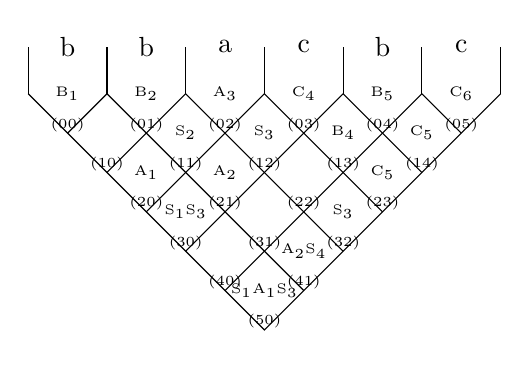
\begin{tikzpicture}[baseline]
		\newcommand{\myfontvars}[1]{
			\fontsize{4.9}{12}\selectfont{#1}
		}\newcommand{\myfontnumbering}[1]{
			\fontsize{2.5}{12}\selectfont{#1}
		}%Outer hull
		%Tip of the pyramid
		\coordinate (tip) at (3.0,-3.0);
		\foreach \i in {0,...,6} {
			\coordinate (\i) at (\i,0);
		}
		%Draw the left and right line of the pyramid pointing downwards
		\draw (0) -- (tip) -- (6);
		%Grid lines direction down-left to top-right
		\coordinate (dl1) at (0.5,-0.5);
		\coordinate (dl2) at (1.0,-1.0);
		\coordinate (dl3) at (1.5,-1.5);
		\coordinate (dl4) at (2.0,-2.0);
		\coordinate (dl5) at (2.5,-2.5);
		\draw (dl1) -- (1,0);
		\draw (dl2) -- (2,0);
		\draw (dl3) -- (3,0);
		\draw (dl4) -- (4,0);
		\draw (dl5) -- (5,0);
		%Grid lines direction down-right to top-left
		\coordinate (dr1) at (3.5,-2.5);
		\coordinate (dr2) at (4.0,-2.0);
		\coordinate (dr3) at (4.5,-1.5);
		\coordinate (dr4) at (5.0,-1.0);
		\coordinate (dr5) at (5.5,-0.5);
		\draw (dr1) -- (1,0);
		\draw (dr2) -- (2,0);
		\draw (dr3) -- (3,0);
		\draw (dr4) -- (4,0);
		\draw (dr5) -- (5,0);
		%Small lines at the top
		\coordinate (top0) at (0.0,0.0);
		\coordinate (top1) at (1.0,0.0);
		\coordinate (top2) at (2.0,0.0);
		\coordinate (top3) at (3.0,0.0);
		\coordinate (top4) at (4.0,0.0);
		\coordinate (top5) at (5.0,0.0);
		\coordinate (top6) at (6.0,0.0);
		\coordinate (topUpper0) at (0.0,0.6);
		\coordinate (topUpper1) at (1.0,0.6);
		\coordinate (topUpper2) at (2.0,0.6);
		\coordinate (topUpper3) at (3.0,0.6);
		\coordinate (topUpper4) at (4.0,0.6);
		\coordinate (topUpper5) at (5.0,0.6);
		\coordinate (topUpper6) at (6.0,0.6);
		\draw (top0) -- (topUpper0);
		\draw (top1) -- (topUpper1);
		\draw (top2) -- (topUpper2);
		\draw (top3) -- (topUpper3);
		\draw (top4) -- (topUpper4);
		\draw (top5) -- (topUpper5);
		\draw (top6) -- (topUpper6);
		%The string
		\coordinate (w0) at (0.5,0.6);
		\coordinate (w1) at (1.5,0.6);
		\coordinate (w2) at (2.5,0.6);
		\coordinate (w3) at (3.5,0.6);
		\coordinate (w4) at (4.5,0.6);
		\coordinate (w5) at (5.5,0.6);
		\node [] at (w0) {b};
		\node [] at (w1) {b};
		\node [] at (w2) {a};
		\node [] at (w3) {c};
		\node [] at (w4) {b};
		\node [] at (w5) {c};
		% Variables in the cells
		%cells00
		\coordinate (center00) at (0.5,0.0);
		\node [below=0.18cm] at (center00) {\myfontnumbering{$(00)$}};
		\node [] at (center00) {\myfontvars{B$_{1}$}};
		%cells01
		\coordinate (center01) at (1.5,0.0);
		\node [below=0.18cm] at (center01) {\myfontnumbering{$(01)$}};
		\node [] at (center01) {\myfontvars{B$_{2}$}};
		%cells02
		\coordinate (center02) at (2.5,0.0);
		\node [below=0.18cm] at (center02) {\myfontnumbering{$(02)$}};
		\node [] at (center02) {\myfontvars{A$_{3}$}};
		%cells03
		\coordinate (center03) at (3.5,0.0);
		\node [below=0.18cm] at (center03) {\myfontnumbering{$(03)$}};
		\node [] at (center03) {\myfontvars{C$_{4}$}};
		%cells04
		\coordinate (center04) at (4.5,0.0);
		\node [below=0.18cm] at (center04) {\myfontnumbering{$(04)$}};
		\node [] at (center04) {\myfontvars{B$_{5}$}};
		%cells05
		\coordinate (center05) at (5.5,0.0);
		\node [below=0.18cm] at (center05) {\myfontnumbering{$(05)$}};
		\node [] at (center05) {\myfontvars{C$_{6}$}};
		%cells10
		\coordinate (center10) at (1.0,-0.5);
		\node [below=0.18cm] at (center10) {\myfontnumbering{$(10)$}};
		%cells11
		\coordinate (center11) at (2.0,-0.5);
		\node [below=0.18cm] at (center11) {\myfontnumbering{$(11)$}};
		\node [] at (center11) {\myfontvars{S$_{2}$}};
		%cells12
		\coordinate (center12) at (3.0,-0.5);
		\node [below=0.18cm] at (center12) {\myfontnumbering{$(12)$}};
		\node [] at (center12) {\myfontvars{S$_{3}$}};
		%cells13
		\coordinate (center13) at (4.0,-0.5);
		\node [below=0.18cm] at (center13) {\myfontnumbering{$(13)$}};
		\node [] at (center13) {\myfontvars{B$_{4}$}};
		%cells14
		\coordinate (center14) at (5.0,-0.5);
		\node [below=0.18cm] at (center14) {\myfontnumbering{$(14)$}};
		\node [] at (center14) {\myfontvars{C$_{5}$}};
		%cells20
		\coordinate (center20) at (1.5,-1.0);
		\node [below=0.18cm] at (center20) {\myfontnumbering{$(20)$}};
		\node [] at (center20) {\myfontvars{A$_{1}$}};
		%cells21
		\coordinate (center21) at (2.5,-1.0);
		\node [below=0.18cm] at (center21) {\myfontnumbering{$(21)$}};
		\node [] at (center21) {\myfontvars{A$_{2}$}};
		%cells22
		\coordinate (center22) at (3.5,-1.0);
		\node [below=0.18cm] at (center22) {\myfontnumbering{$(22)$}};
		%cells23
		\coordinate (center23) at (4.5,-1.0);
		\node [below=0.18cm] at (center23) {\myfontnumbering{$(23)$}};
		\node [] at (center23) {\myfontvars{C$_{5}$}};
		%cells30
		\coordinate (center30) at (2.0,-1.5);
		\node [below=0.18cm] at (center30) {\myfontnumbering{$(30)$}};
		\node [] at (center30) {\myfontvars{S$_{1}$S$_{3}$}};
		%cells31
		\coordinate (center31) at (3.0,-1.5);
		\node [below=0.18cm] at (center31) {\myfontnumbering{$(31)$}};
		%cells32
		\coordinate (center32) at (4.0,-1.5);
		\node [below=0.18cm] at (center32) {\myfontnumbering{$(32)$}};
		\node [] at (center32) {\myfontvars{S$_{3}$}};
		%cells40
		\coordinate (center40) at (2.5,-2.0);
		\node [below=0.18cm] at (center40) {\myfontnumbering{$(40)$}};
		%cells41
		\coordinate (center41) at (3.5,-2.0);
		\node [below=0.18cm] at (center41) {\myfontnumbering{$(41)$}};
		\node [] at (center41) {\myfontvars{A$_{2}$S$_{4}$}};
		%cells50
		\coordinate (center50) at (3.0,-2.5);
		\node [below=0.18cm] at (center50) {\myfontnumbering{$(50)$}};
		\node [] at (center50) {\myfontvars{S$_{1}$A$_{1}$S$_{3}$}};
		\end{tikzpicture}
	}
	\end{minipage}
	\captionof{figure}{The CYK algorithm fills the cells of the pyramid during execution of Line \ref{fill1} and Line \ref{fill2}.}
	\label{exampleCYK}
\end{testexample}


\clearpage
\pagebreak